\section{Umfrage}

\subsection{Frage 1}
\begin{center}
	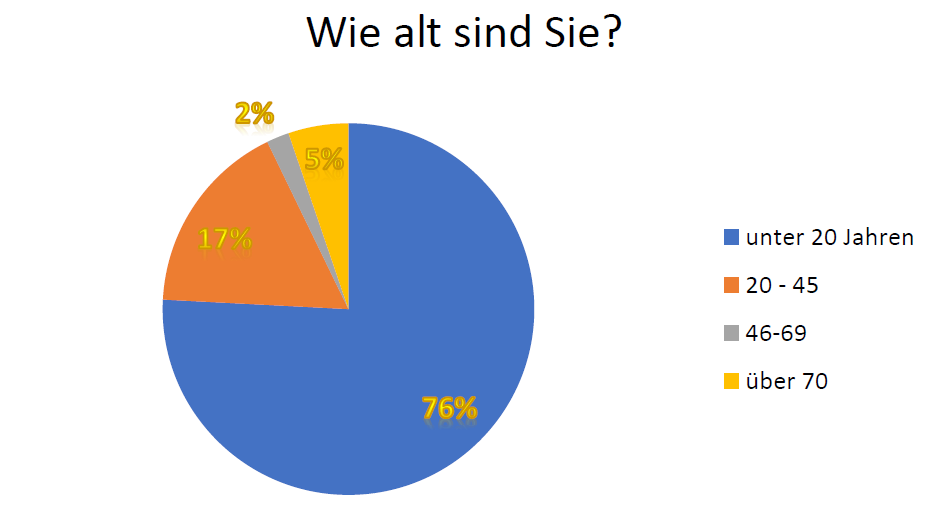
\includegraphics[width=0.8\textwidth]{./img/umfrage1}
	\captionof{figure}{\label{fig:Frage1}Umfrage - Frage 1}
\end{center}
An der Umfrage haben insgesamt 120 Personen teilgenommen. Davon waren 76\% unter 20 Jahren, 17\% 20 bis 45 Jahre, 2\% 46 bis 69 Jahre und 5\% über 70 Jahre alt.

\subsection{Frage 2}
\begin{center}
	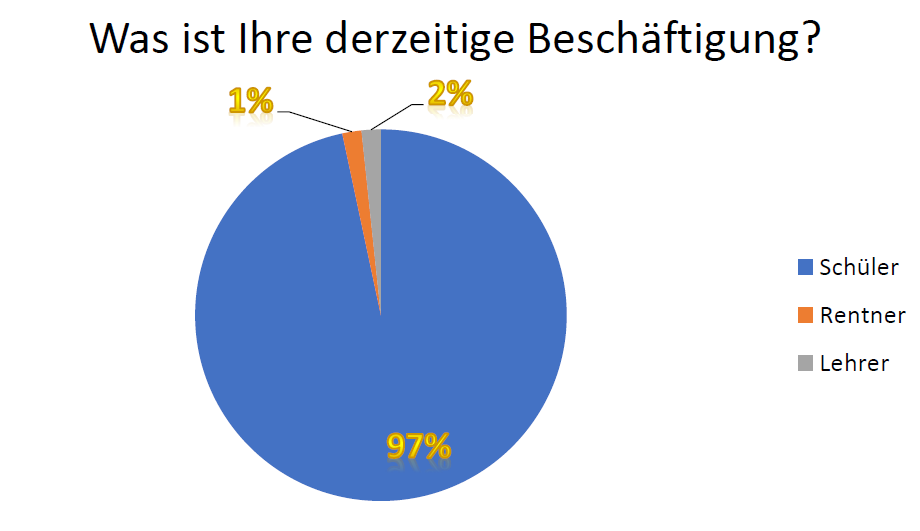
\includegraphics[width=0.8\textwidth]{./img/umfrage2}
	\captionof{figure}{\label{fig:Frage2} Umfrage - Frage 2}
\end{center}
Von den Befragten waren 97\% Schüler, 1\% Rentner und 2\% Lehrer.


\subsection{Frage 3}
\begin{center}
	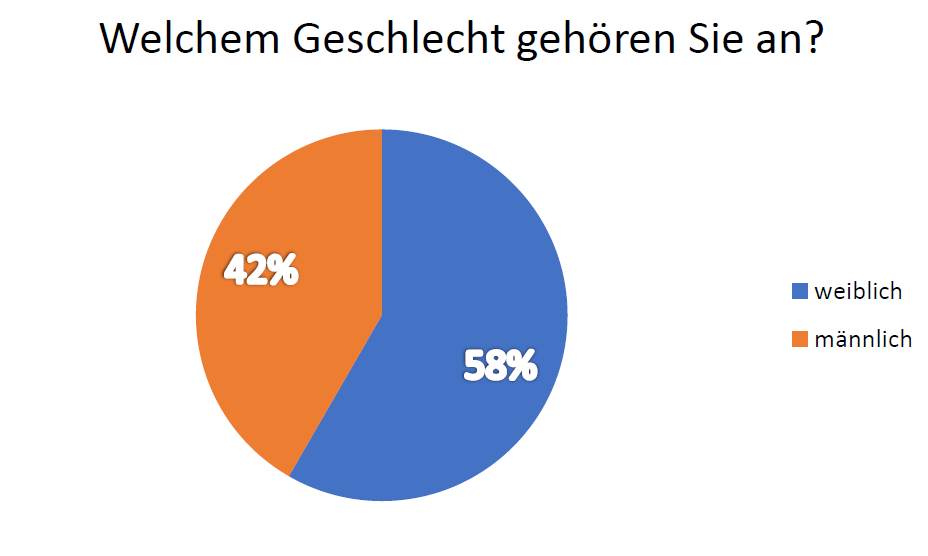
\includegraphics[width=0.8\textwidth]{./img/umfrage3}
	\captionof{figure}{\label{fig:Frage3} Umfrage - Frage 3}
\end{center}
An der Umfrage haben mehr Frauen (58\%) teilgenommen als Männer (42\%).

\subsection{Frage 4}
\begin{center}
	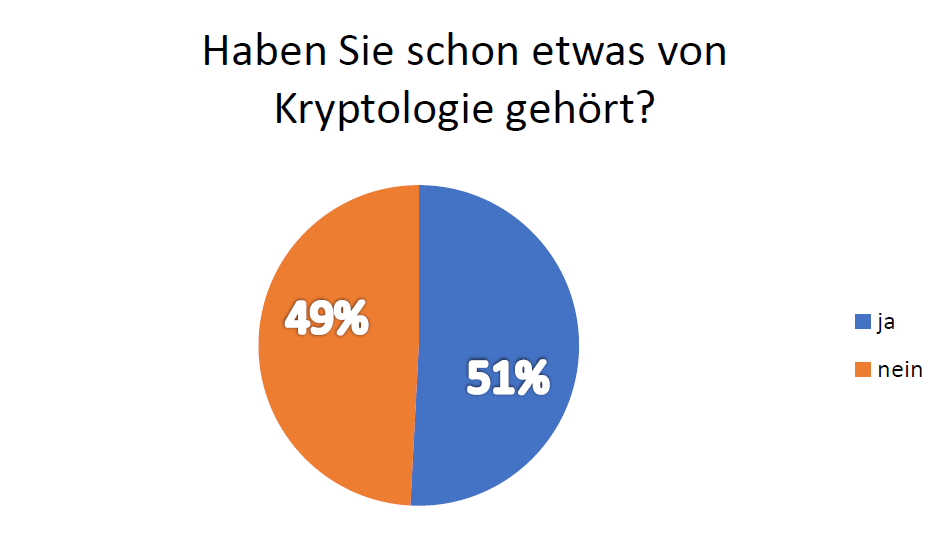
\includegraphics[width=0.8\textwidth]{./img/umfrage4}
	\captionof{figure}{\label{fig:Frage4} Umfrage - Frage 4}
\end{center}
51\% der Personen haben zuvor schon einmal etwas über Kryptologie gehört und 49\% konnten sich darunter nichts vorstellen.

\subsection{Frage 5}
\begin{center}
	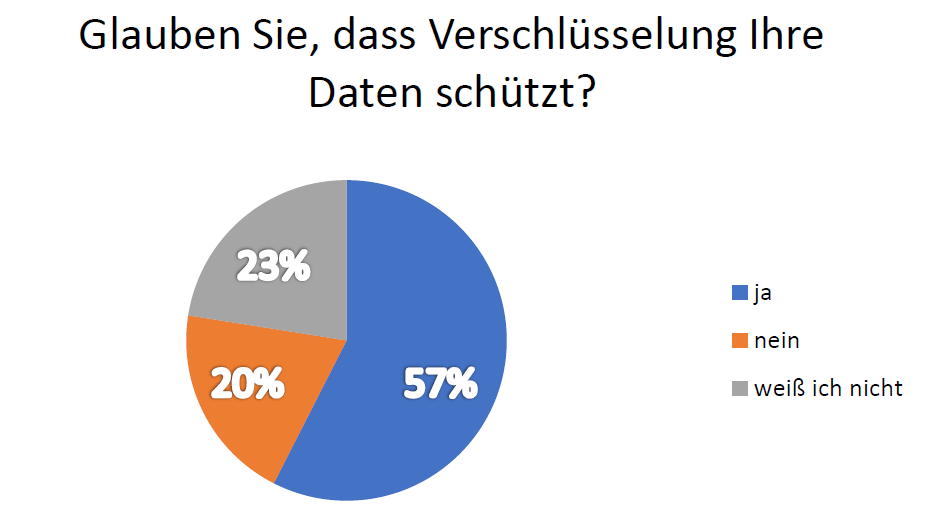
\includegraphics[width=0.8\textwidth]{./img/umfrage5}
	\captionof{figure}{\label{fig:Frage5} Umfrage - Frage 5}
\end{center}
Bei der Umfrage gaben 57\% an, dass eine Verschlüsselung die Daten schützen kann. 20\% glaubten nicht das dies der Fall ist und 23\% gaben an, dass sie das nicht wüssten.


\subsection{Frage 6}
\begin{center}
	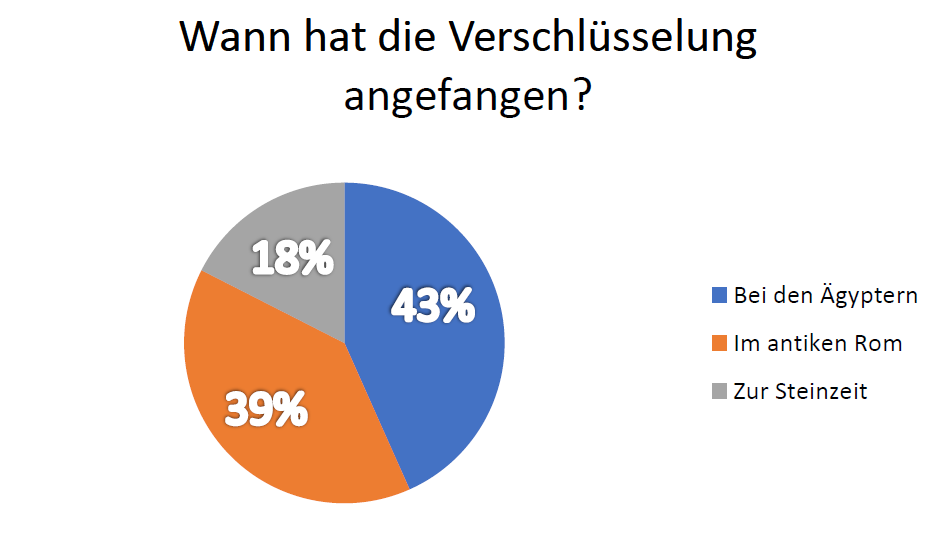
\includegraphics[width=0.8\textwidth]{./img/umfrage6}
	\captionof{figure}{\label{fig:Frage6} Umfrage - Frage 6}
\end{center}
Bei der Frage: Wann hat die Verschlüsselung angefangen gaben 43\% bei den Ägyptern, 39\% im antiken Rom und 18\% zur Steinzeit an.


\subsection{Frage 7}
\begin{center}
	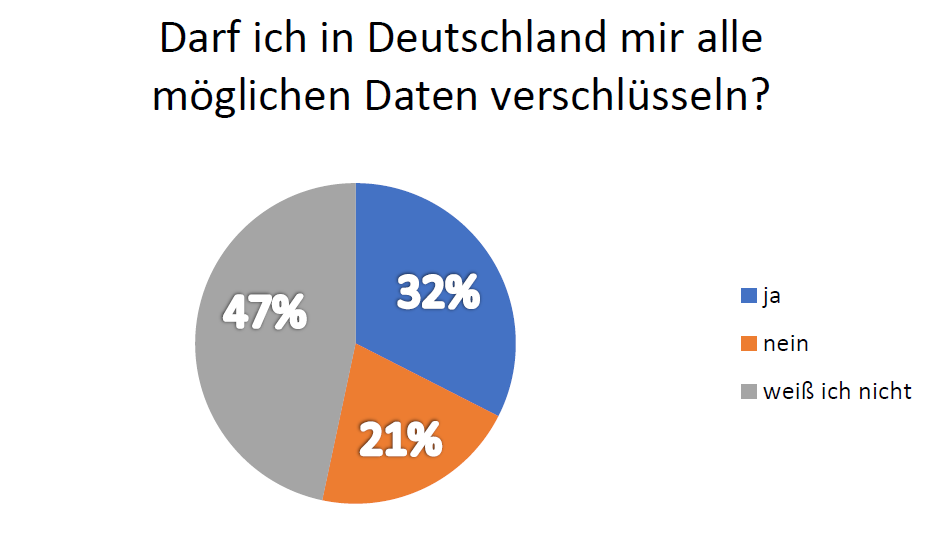
\includegraphics[width=0.8\textwidth]{./img/umfrage7}
	\captionof{figure}{\label{fig:Frage7} Umfrage - Frage 7}
\end{center}
Es gaben 32\% an, dass man alle möglichen Daten in Deutschland verschlüsseln darf. 21\% der Befragten gaben nein an. Und 47\% gaben an, dass Sie nicht darüber wissen.



\subsection{Frage 8}
\begin{center}
	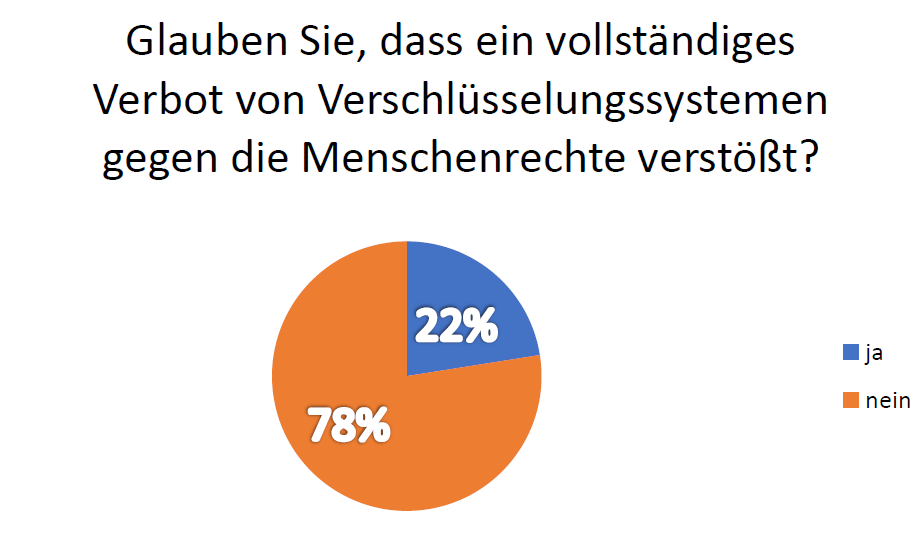
\includegraphics[width=0.8\textwidth]{./img/umfrage8}
	\captionof{figure}{\label{fig:Frage8} Umfrage - Frage 8}
\end{center}
Es gaben 32\% an, dass man alle möglichen Daten in Deutschland verschlüsseln darf. 21\% der Befragten gaben nein an. Und 47\% gaben an, dass Sie nicht darüber wissen.
78\% der Befragten gaben an, dass es nicht gegen die Menschenrechte verstoßen würden und 22\% sagten, dass es gegen die Menschenrechte verstößt.

\subsection{Frage 9}
\begin{center}
	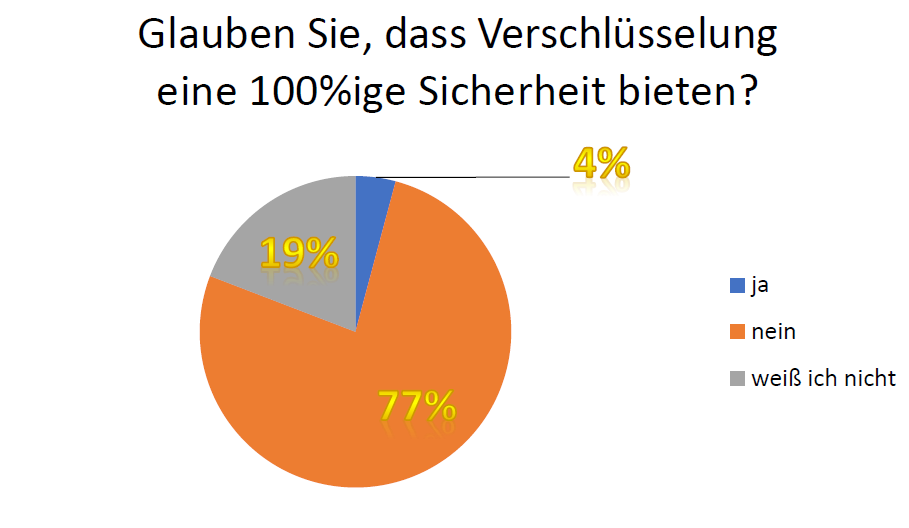
\includegraphics[width=0.8\textwidth]{./img/umfrage9}
	\captionof{figure}{\label{fig:Frage9} Umfrage - Frage 9}
\end{center}
Bei der Frage: Glauben Sie, dass Verschlüsselung eine 100\%ige Sicherheit bieten, gaben 4\% ja, 77\% nein und 19\% weiß ich nicht an.

\subsection{Frage 10}
\begin{center}
	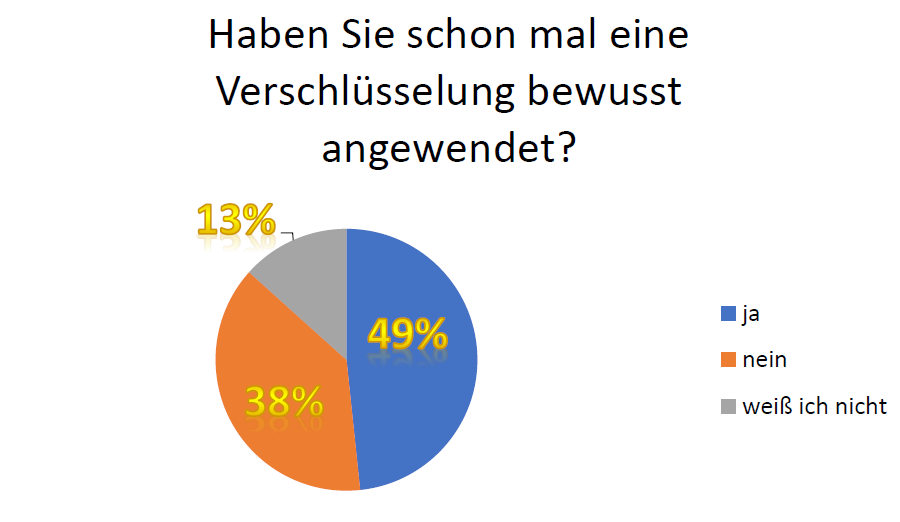
\includegraphics[width=0.8\textwidth]{./img/umfrage10}
	\captionof{figure}{\label{fig:Frage10} Umfrage - Frage 10}
\end{center}
Bei dieser Frage gaben 49\% ja, 38\% nein und 13\% weiß ich nicht an.
